\namedsection{FPGA}{Pasat}

The FPGA was initially designed to have a Cortex-M0\_DS processor, a block of memory with a program that fetches constants from that block at regular intervals, a reset and a pattern detector attached to the bus so when a specific pattern appears on the data bus, the LED turns on and when another patters appears it will turn off. The Cortex-M0\_DS  includes only the processor and a non-synthesisable testbench. Other parts will need to be implemented in order to create a synthesisable system: a software executable image, a system clock, a detector module for the command LED and a reset synchroniser. This section will be divided into: software development and simulation, system implementation and functional simulation. All of these sections will be discussed in detail in what follows.

\begin{figure}
	\centering
	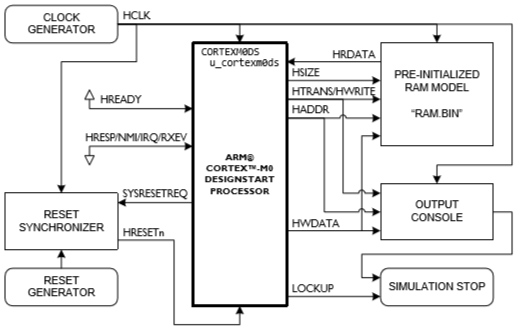
\includegraphics[scale=0.7]{figures/test_bench_schematic.PNG}
	\caption{Cortex M0 test bench schematic} \label{fig:test_bench}
\end{figure}

Through ARM, access was obtained to a fixed configuration of the Cortex-M0 Processor known as Cortex-M0 DesignStart \cite{armdesignstart}. This simplified version offers us access to a Verilog version of the Cortex-M0 under the form of an obfuscated and preconfigured netlist, but it can be synthesised. This package also includes a test-bench which allows for simulation of the Cortex-M0 DesignStart module connected to a memory model and a clock and reset generator. It also includes a basic C \verb|helloworld.c| program. The schematic for the test-bench can be seen in figure \ref{fig:test_bench} and it connects the CORTEXM0DS to a memory model, a clock and a reset generators.

ModelSim was used for running the test-bench, which is a tool that offers the possibility of simulating hardware description languages such as Verilog and VHDL.  A memory image, provided within the DesignStart package, is used for the \verb|helloworld.c| program, which is used by the test-bench to write a message to the simulator's console and after that end the simulation. 

Also, access was given to the CM0DS example design kit which contains various AHB-Lite peripherals and infrastructure components, useful to create complete systems. Before implementing the actual algorithm on the FPGA, a more basic simulation needs to be conducted on the platform to assure that it is compatible with the specific FPGA used. Next, the analysis of the sensors used for our project will be discussed. 


\subsection{Software development and simulation}
In this section, a software program that will verify the memory fetches of some predefined constants. The program used for this will be the IDE ARM Keil $\mu$Vision which allows quick and easy building of projects.

To start, a new project must be created in $\mu$Vision. Next, the device must be selected device database so ARM-ARM Cortex M0 plus-ARMCM0P is selected which can be seen in figure \ref{fig:armcm0p}.

\begin{figure}
\centering
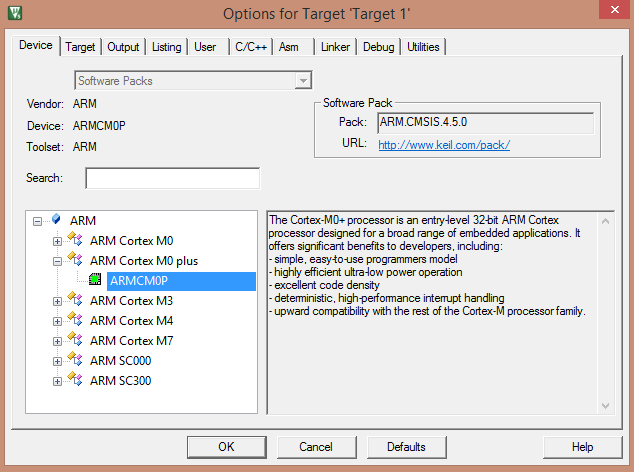
\includegraphics[scale=0.7]{figures/armcm0p.PNG}
\caption{Selection of the Cortex M0+ for the μVision project} 
\label{fig:armcm0p}
\end{figure}

After this is selected, the options menu is accessed for this device. Next, the target options need to be accessed and the following modification need to be made:

- under Target section, the Read/Write Memory Areas, RAM1 starts at 0x0 and has the size of 0x400000 (this setting is used to create a linker scatter file. Another requirement for this is the having the Use Memory Layout from Target Dialog enabled in the Linker section);

- under Output section, the Debug Information and Browse Information sections need to be ticked(this defines the resulting output files from the tool chain and allows the user programs to be started after the building process is complete);

- under Listing section, all the default selected features stay the same(here all the listing files generated by the tool chain are specified);

- under User section, in Run\#1:"fromelf -cvf code.axf --vhx --32x1 -o code.hex" and Run\#2:"fromelf -cvf code.axf -o disasm.txt" in Run User Programs After Build/Rebuild those code lines are inserted in order to create a .axf file from the .hex file;

- under C/C++ section, the One ELF Section per Function is unticked and the Warnings are set to "unspecified" (here C/C++ specific tool options are set);

-under Asm section, all the settings are kept to default also(this allows the setting of specific Assembler tool options);

-under Linker section, the R/W Base entry is deleted and only the R/O Base: 0x00000000 remains(linker settings are required in order to configure the physical memory location of the target). The location of memory classes and sections is defined here.

-under Debug section, the default settings for µVision4 Debugger stay the same;

-under Utilities, the Use Target Driver for Flash Programming in the Configure Flash Menu Command is left checked.

\begin{lstlisting}[caption={Reset Handler},label={lst:reset-handler}]
Reset_Handler	PROC
		GLOBAL Reset_Handler
		ENTRY

AGAIN		LDR	R1, =0x50000000		;Write to LED with value 0x55
		LDR	R0, =0x55
		STR	R0, [R1]


		LDR	R0, =0x2FFFFF		;Delay
Loop		SUBS	R0,R0,#1
		BNE Loop

		LDR	R1, =0x50000000		;Write to LED with value 0xAA
		LDR	R0, =0xAA
		STR	R0, [R1]

		LDR	R0, =0x2FFFFF		;Delay
Loop1		SUBS	R0,R0,#1
		BNE Loop1
\end{lstlisting}

After all of these steps have been done, it is now time to add the assembly file provided by ARM, the \verb|cm0dasm.s| to the source. Taking a look at the reset handler, which can be seen in \ref{lst:reset-handler}, it turns on half of the 8-bit LEDs (for example 0, 2, 4 ,6), sets up a counter and uses it for a short time delay, then turns on the other half and delays another period.

After the successful building, the code.hex should be created and converted into a .axf because it was set in the User section. The .axf file needs to be converted to a .bin in order to program the FPGA. The MDK/Keil offers a tool called "fromelf" which can do this conversion. It is called in the following way:

fromelf --bin --o code.bin code.axf

This can be used to program the FPGA. Now, the implementation of the Cortex-M0 will be discussed.

\subsection{System Implementation}

The simulated ARM Cortex-M0 processor includes the AHB-Lite system bus and two AHB peripherals: the program memory (which will be implemented using on-chip memory blocks) and a simple LED peripheral. Some of the steps are similar for implementing the Cortex M0 on a older FPGA~\cite{implementationcortexm0onnexys2}, but since different modules and software are required, some of the same steps may not apply.

The software used for this implementation was Vivado Design Suite produced by Xilinx. This is used for synthesis and analysis of HDL designs. It is a improved version of the Xilinx ISE which also allows features such as system on a chip development and a high-level synthesis. 

The Cortex-M0 DesignStart will be used, which is a simplified version of the industry Cortex-M0 processor, but has some features reduced which are not essential for this project such as the number of available interrupts (from 32 to 16). Two verilog files are included in this pack:  \verb|cortexm0ds_logic.v| and \verb|CORTEM0DS.v|. The \verb|cortexm0ds_logic.v| contains the Cortex-M0 DesignStart processor logic level Verilog file, while the CORTEXM0DS.v includes the Cortex-M0 DesignStart processor macro cell level.

On-chip memory block are used in order to implement the program memory in SoC, for example the Block RAM (BRAM) which is present on this FPGA. The program image needs to be merged into the hardware design during synthesis to load the program on the on-chip memory of the FPGA.

Now, in order to implement the Cortex M0 on the FPGA, more than just the ARM DesignStart Verilog codes are necessary. The ARM Cortex-M System Design Kit (CMSDK) contains a set of \verb|AMBA|, \verb|AHB| and \verb|APB| components and examples for various Cortex-M systems processors, including the Cortex-M0. The  Verilog file  used from this package in order to reproduce the desired experiment will be discussed.

The \verb|AHBDCD.v| contains the code for the address decoder of the \verb|AHB| bus. This uses a Multi-layer bus architecture having only one \verb|AHB| master on each of the input layers and one \verb|AHB| slave on each of the outputs, the entire system address decoding can be done within the decoder section. 

The \verb|AHBMUX.v| contains the code for the slave multiplexor of the \verb|AHB| bus. This uses parameters in order to specify the slave port usage in order for the synthesis process to no generate extra logic which is not necessary for the project. The slave to master multiplexer controls the response signals and read data routing from the bus slaves to the bus masters. The address decoder presented earlier is used to determine the currently selected slave and generates the \verb|HSEL| signal to the \verb|AHB| slaves and slave multiplexer. The multiplexer creates the connection between the slave outputs and the inputs of the bus masters. 

\begin{figure}
\centering
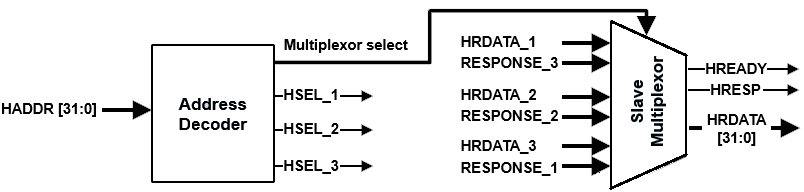
\includegraphics[scale=0.7]{figures/decoder_and_multiplexer.PNG}
\caption{Address Decoder and Slave Multiplexor\cite{ahblite} } 
\label{fig:decoder_multiplexer}
\end{figure}

Figure \ref{fig:decoder_multiplexer} shows how two Address Decoder and Slave Multiplexor can be seen. The \verb|HADRR|[0:31] signal sends the read data from multiplexer to master \cite{ahblite}. The \verb|HREADY| signal goes from the multiplexor to the master and slaves and when it is set to HIGH, it indicates that the previous transfer has been completed. The \verb|HRESP| signal transfers the response signal from multiplexor to master. Each of the slaves has its own select signal \verb|HSEL| which indicates the current transfer intended for that specific slave. Before being able to respond to the current transfer, the status of \verb|HREADY| must be known in order to ensure that the previous transfer has been completed. 

The \verb|AHB2BRAM.v| contains the on-chip memory peripheral (BRAM) 
which is a configurable memory module that gives access to a variety of BRAM Interface Controllers. This is used for the program memory of the processor.

The \verb|AHB2LED.v| contains the LED peripheral module. Selected LED will light up when a specific generated patters will be detected and will turn off when another pattern is detected.

The \verb|AHBLITE_SYS.v| contains the top-level module. The AHB-Lite is a subset of the full \verb|AHB| specification which is used in designs where there is no more than one bus master used. This simplifies the \verb|AHB| specification because it removes the unnecessary protocol used for more bus masters.

The \verb|ARMSOC_s6.ucf| file is the user constraint file which creates the connection between the assigned nets and FPGA pins.

All of these files files need to be added to a Vivado project in order to create and download the bitstream file to the FPGA. A new project was created, specifying that it is a RTL project. A mixed implementation setting between Verilog/VHDL will be required for this project. The processor is described in Verilog while the additional modules are in VHDL. Next, in the list of Xilinx parts, the XC7A100T-1CSG324C needs to be selected because this is the part name for the Nexys4 board. 

\begin{figure}
\centering
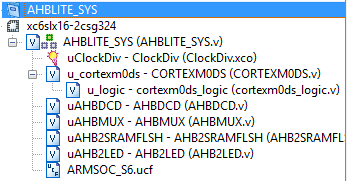
\includegraphics[scale=0.7]{figures/AHBLITE_SYS_modules_ISE_schematic.PNG}
\caption{AHB Lite top-module } 
\label{fig:ahblite_sys}
\end{figure}

After the project is created, the \verb|AHBALITE_SYS.v| is set as a top module since this creates the connection between all the components. This can be seen in \ref{fig:ahblite_sys}. Because this is a Nexys4 board and the Clock Divider supplied in the package are not compatible due to the fact that it requires a Spartan 6 Series processor, a new IP needed to be created for this specific FPGA. In order to add this we need to go to Source-New Source-IP CORE(Generator and Architecture Wizard)-Clocking-Clocking Wizard. This is going to generate a system clock at 10MHz from the board's 50MHz external oscillator. In figure \ref{fig:clock}, the Input Clock Frequency is set 50 MHz and the Output Frequency to 10 MHz and it is named "uClockDiv".

\begin{figure}
\centering
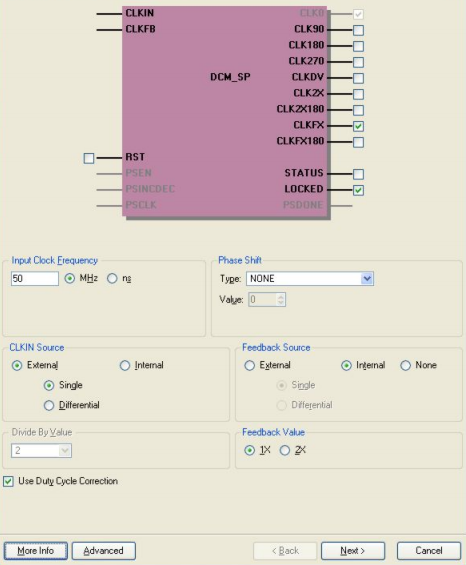
\includegraphics[scale=0.7]{figures/clock_creation.PNG}
\caption{Clocking Wizard settings } 
\label{fig:clock}
\end{figure}

Since the user constraint file supplied is meant to be used to a Spartan 6 Series FPGA board, the user constraint file needed modifications in order to fit the Artix-7 FPGA. The UCF can be seen in appendix \ref{ch:ucffile}. After this, the top module of the simulation can be implemented and translated int o a .bit file which is used to program the FPGA.

\subsection{Functional Simulation}
Due to some unplanned delays in acquiring certain documentations, delays in obtaining licenses for the various software used and difficulties encountered during the creation of a proper .bit file, a full functional simulation was not properly conducted. A basic simulation of the Cortex M0 was presented in \ref{sec:cortex}.  The functional simulation of the system verifies if the signal in HRDATA are the ones expected and if it works as expected. Vivado Hardware Debug is the Vivado tool used for debugging. This is accessed by going to Design-View:Simulation. If a complete functional would have been performed, a run-time simulation needs to also be performed. On-chip debugging tools such as ChipScope are required in order to perform this sort of simulation. Inside the analysis, these AHB signals need to be evaluated to see if they work correspondingly: 
HADDR[31:0] 
HWDATA[31:0]
HRDATA[31:0]
HWRITE
HREADY
HSIZE[2:0]
HTRANS[1:0]
HRESP

\subsection{Decision on final prototype}
The team decided that the mBed platform had a better progress and would be more suitable for our final design since it's small size will allow strapping it people, opposed to the FPGA board which was much greater in size. Because of this, I stopped attempting to implement the Cortex M0 and redirected my attention to other aspects of the project where is was more necessary. Next, the successful section prototype of our project which was implemented on the mBed will be discussed.
